\normaltrue \difficilefalse \tdifficilefalse
\correctionfalse

%\UPSTIidClasse{11} % 11 sup, 12 spé
%\newcommand{\UPSTIidClasse}{12}

\exer{Système bielle manivelle  $\star\star$ \label{C2:06:12}}
\setcounter{numques}{0}
\UPSTIcompetence[2]{C2-06}
\index{Compétence C2-06}
\index{Bielle Manivelle}
\index{Moteur}
\ifcorrection
\else
\textbf{Pas de corrigé pour cet exercice.}
\fi

\ifprof
\else
Soit le mécanisme suivant. On a $\vect{AB}=R\vect{i_1}$, $\vect{CB}=L\vect{i_2}$ et $\vect{AC}=\lambda(t) \vect{j_0}$. 

\begin{center}
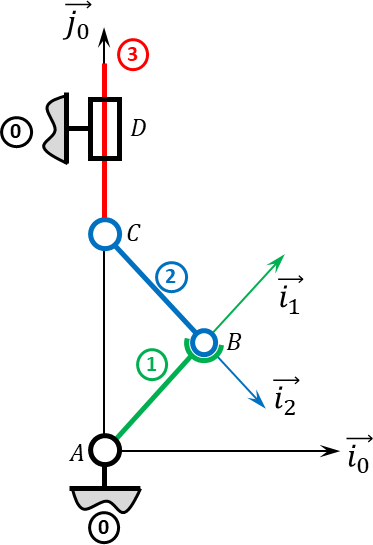
\includegraphics[width=\linewidth]{12_01}
\end{center}
\fi

\question{Tracer le graphe des liaisons.}
\ifprof
\else
\fi

\question{Exprimer $\lambda(t)$ en fonction de $\theta(t)$.}
\ifprof
\else
\fi

\question{Exprimer $\dot{\lambda}(t)$ en fonction de $\dot{\theta}(t)$.}
\ifprof
\else
\fi

\question{En utilisant Python, tracer la vitesse du piston en fonction du temps. La fréquence de rotation est $\dot{\theta}(t)=\SI{100}{rad.s^{-1}}$, on prendra $R=\SI{10}{mm}$ et $L=\SI{10}{mm}$, puis $L=\SI{20}{mm}$ et $L=\SI{30}{mm}$.}
\ifprof
\else
\fi

\question{En utilisant Python, tracer l'accélération du piston en fonction du temps en utilisant les mêmes valeurs que dans la question précédente. On utilisera une dérivation numérique.}
\ifprof
\else
\fi


\ifprof
\else
\begin{flushright}
\footnotesize{Corrigé  voir \ref{C2:06:12}.}
\end{flushright}%
\fi